\documentclass[dvipdfmx]{standalone}
\usepackage{graphicx}
\usepackage{tikz}
\usetikzlibrary{arrows.meta, calc}
\begin{document}
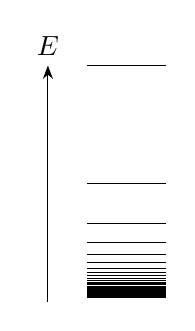
\begin{tikzpicture}
    \draw[->, >=Stealth](0,0)--(0,3)node[above]{$E$};
    % \draw(.5,0)--++(1,0);
    \foreach\y in{1,2,...,50}{
        \draw(.5,{3/\y})--++(1,0);
    }
\end{tikzpicture}
\end{document}
